\subsection{Database Paket Implementierungsänderungen}
\paragraph{TemplateData} Die Klasse TemplateData des Database Pakets wurde entfernt da es keine Einträge in der Datenbank gibt die sie verwalten muss\ref{template_gone}.


\paragraph{DatabaseTable} Unterscheidung zwischen einzelnen Werten und Mehreren für get(..) Funktion. Dadurch entstehen get\textunderscore one(..) und get\textunderscore multiple(..).

Neue Funktion \textbf{check\textunderscore for(query: str): bool} um zu sehen ob ein Eintrag von der angegebenen query existiert.

Neue Funktion \textbf{setup\textunderscore database()} die beim Aufrufen die Datenbank aufbaut

\paragraph{WorkflowData} Hauptsächlich Typisierung und Namensgebung 

\newline

\subsection{MySQL - Datenbankaufbau}

\begin{figure}[h]
	\centering
	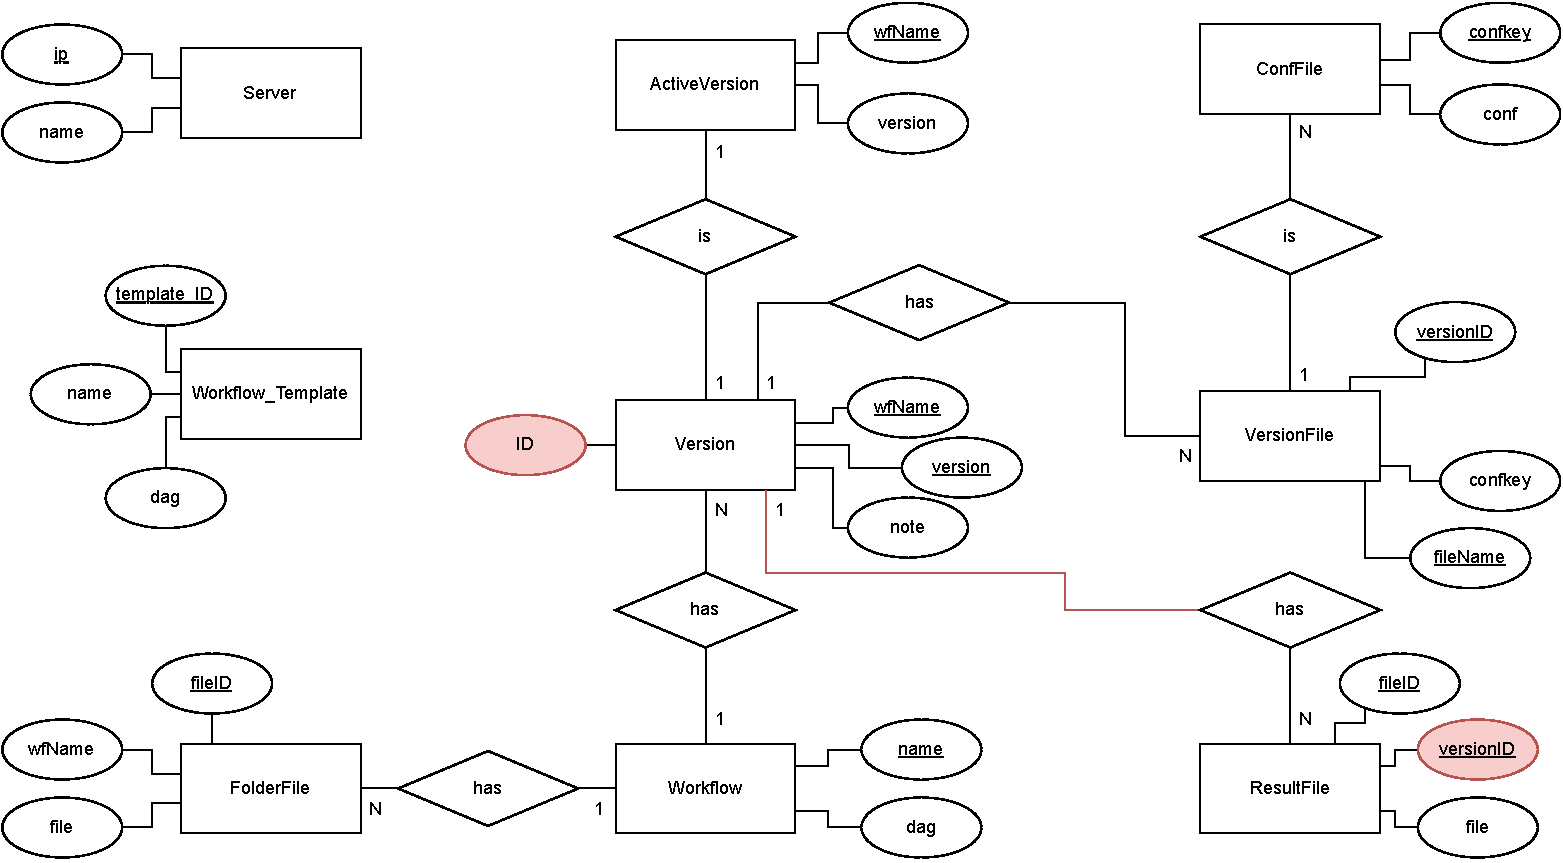
\includegraphics[width=0.85\textwidth]{res/er_diagram.pdf} 
	\caption{ER-Diagramm der Datenbank. Änderungen in rot}
	\label{fig:er_diagram}
\end{figure}

Auf \ref{fig:er_diagram} ist das Überarbeitete ER-Diagramm der Datenbank zu sehen.

Nach langen Überlegungen sind wir zu dem Schluss gekommen, dass es sinnvoller ist für die Dateispeicherung statt LONGBLOBS und weitere Parameter, nur Pfade in die Datenbank einzuspeichern, die auf die gewünschte Datei zeigen. Zum einen gibt es dadurch weniger rohe Daten die zwischen (manchen) Funktionen kommuniziert werden müssen, aber auch weniger Latenz beim schreiben oder lesen der Dateien aus der Datenbank.

\label{template_gone}Demzufolge ist es uns möglich Workflow Templates in einem einzigen Ordner zu speichern der alle DAG's beinhaltet die nach ihren Template Namen benannt sind. Dieser Ordner ist leicht zu erreichen und darüber zu iterieren. Die Tabelle Workflow\textunderscore Template\ref{wfTemplate} ist dementsprechend nicht mehr benötigt, da der Ordner als eigene Tabelle fungieren kann. Sie bleibt trotzdem bis auf weiteres in der Datenbank um bei eventuellen Komplikationen schneller wechseln zu können.


Weitere Änderungen beinhalten die Vereinfachung einer Workflow-Version in der Datenbank. Statt zwei Schlüssel 'wfName' und 'version' bekommt jede Version einen eindeutigen Integer Bezeichner. Dieser muss zwar für manche Zugriffe auf andere Tabellen zuerst von Version geholt werden, erhöht aber das Verständnis der Datenbankstruktur und bringt eine Erleichterung der MySQL-Befehle.

Die Verbindung von ResultFile wurde außerdem zu Version geändert. Es besteht keinen Grund das komplexe System der Speicherung von überlappenden .conf Dateien auch für die (höchstwahrscheinlich) immer unterschiedlichen Ergebnisse unterschiedlicher Versionen zu nutzen. Ein einfacher Fremdschlüssel der auf die entsprechende Workflow-Version zeigt reicht aus.


Dementsprechend sind Folgende Tabellen in der Datenbank vorhanden:

\paragraph{}
\begin{dataTable}
	\hline
	\textbf{Server} & & \\
	\hline
	ip & varchar(50) & $key$ \\
	\hline
	name & varchar(255) & $key$ \\
	\hline
\end{dataTable}

\paragraph{}
\begin{dataTable}
	\hline
	\textbf{WorkflowTemplate\label{wfTemplate}} &  & \\
	\hline
	template\textunderscore ID & int & $key; Auto\_Increment$\\
	\hline
	name & varchar(255) & $notNull$ \\
	\hline
	dag & varchar(255) & $notNull$\\
	\hline
\end{dataTable}

\paragraph{}
\begin{dataTable}
	\hline
	\textbf{Workflow} &  & \\
	\hline
	name & varchar(255) & $key$ \\
	\hline
	dag & varchar(255) & $notNull$\\
	\hline
\end{dataTable}

\paragraph{}
\begin{dataTable}
	\hline
	\textbf{FolderFile} &  & \\
	\hline
	filesID & int & $key; Auto\_Increment$ \\
	\hline
	wfname & varchar(255) & $notNull;$ name from Workflow\\
	\hline
	file & varchar(255) & $notNull$\\
	\hline
\end{dataTable}

\paragraph{}
\begin{dataTable}
	\hline
	\textbf{Version} & & \\
	\hline
	ID & int & $key; Auto\_Increment$ \\
	\hline
	wfName & varchar(255) & name from Workflow\\
	\hline
	version & varchar(127) & $notNull$ \\
	\hline
	note & varchar(1000) & \\
	\hline
\end{dataTable}

\paragraph{}
\begin{dataTable}
	\hline
	\textbf{ActiveVersion} & & \\
	\hline
	wfName & varchar(255) & $key;$ name from Workflow\\
	\hline
	version & varchar(127) &  from Version\\
	\hline
\end{dataTable}

\paragraph{}
\begin{dataTable}
	\hline
	\textbf{VersionFile} & & \\
	\hline
	versionID & int & $key;$ ID from Version \\
	\hline
	filename & varchar(255) & $key$\\
	\hline
	confKey & int & $notNull;$ from ConfFiles \\
	\hline
\end{dataTable}

\paragraph{}
\begin{dataTable}
	\hline
	\textbf{ConfFile} & & \\
	\hline
	confKey & int & $key; Auto\_Increment$ \\
	\hline
	file & varchar(255) & $notNull$ \\
	\hline
\end{dataTable}

\paragraph{}
\begin{dataTable}
	\hline
	\textbf{ResultFile} &  & \\
	\hline
	versionID & int & $key;$ ID from Version \\
	\hline
	filesID & int & $key; Auto\_Increment$ \\
	\hline
	file & varchar(255) & $notNull$\\
	\hline
\end{dataTable}














